Edellisessä kappaleessa kuvattu ratkaisu on toiminut kohtalaisen hyvin useamman vuoden ottaen huomioon sen yksinkertaisuuden. Siinä on kuitenkin selkeitä heikkouksia. On selvää esimerkiksi, että alle kolmen senttilitran kaatoja tällä toteutuksella ei käytännössä voi tehdä. Tämä toteutus ei myöskään ota huomioon mitään muita muuttujia mitä juomien kaadossa voi olla halutun juomamäärän lisäksi. Tässä kappaleessa käydään läpi erilaisia ongelmia, joita vanhassa kaatoratkaisussa on ollut.

Eri muuttujien vaikutusta juoman kaatoon on yritetty vähentää käyttämällä aina samanlaisia pulloja, ja sen lisäksi pulloissa kaatonokkia. Tämä helpottaa myös kaatoliikkeen ohjelmointia robotille, kun pullosta tuleva juoman virtaus osuu mukiin helpommin. Virtaus on myös tasaisempi kaatonokkaa käytettäessä. Kaatonokassa on pieni korvausilmaputki, joka tasaa painetta pullon sisä- ja ulkopuolella. Kaatoja pullosta ilman kaatonokkaa ovat simuloineet Geiger et al. Simulaatiosta huomataan, miten normaalisti pullon suusta kaadettaessa ilman pitää virrata kaatoaukosta välillä sisäänpäin. Tämä aiheuttaa nesteen virtaukseen nykivää liikettä, jota ei kaatonokkaa käytettäessä tule korvausilmaputken ansiosta.

\begin{figure}
\begin{center}
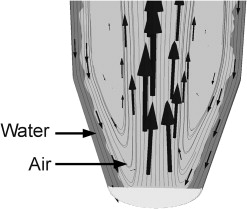
\includegraphics{img/Geiger et al. juoman virtaus.jpg}
\end{center}
\caption{Juoman virtaus}
\label{fig:juomien_virtaus}
% -> \ref{fig:juomien_virtaus}
\end{figure}

Varsinkin kapeilla ulostuloputkilla ilmavirtaus juoman virtausta vastaan tekee juoman virtauksesta huomattavasti turbulenttisemman, mikä vaikuttaa juoman virtausnopeuteen. \cite{Geiger2012} Kapea ulostuloputki on parempi, sillä silloin robotin on paljon helpompi osua lasiin juomaa kaataessa.

\begin{center}
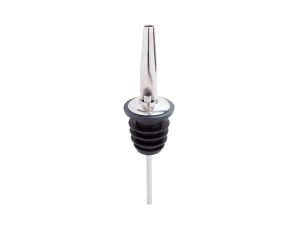
\includegraphics{img/kaatonokka_nettikauppa.jpg}
\end{center}

Juoman kaatamisessa robotilla on kuitenkin omat ongelmansa, vaikka käytössä olisikin kaatonokka. Suurin ongelmista tässä sovelluskohteessa on se, että korvausilmaputkeen saattaa mennä pisara nestettä. Näin pullon sisään ei tule korvausilmaa, ja kaatonokasta ei virtaa nestettä liian suuren paine-eron takia, vaikka pullo olisi kokonaan ylösalaisin. Tällaista tilannetta ei robotti ole osannut havaita. Sen takia asiakkaan lasi on jäänyt käytännössä tyhjäksi ja juomatilaus on jouduttu tekemään uudelleen. Tavoite uudelle kaatoratkaisulle on tällaisen tilanteen tunnistaminen ja siitä palautuminen.

Juomien kaatoon muuttujia tuo huomattavasti lisää myös se, millaista juomaa kaadetaan. Veden, mehujen ja muiden kuohumattomien ja viskositeetiltään samankaltaisten juomien kaataminen onnistuu vielä melko hyvin lineaarisen funktion mukaan, mutta ongelmia alkaa tulla varsinkin kuohuvien juomien kanssa. Tällöin saman lineaarisen funktion käyttö ei enää toimi, sillä esimerkiksi kuplat aiheuttavat turbulenssia kaadon aikana. Vettä paljon suuremman viskositeetin omaavat nesteet ovat dynamiikaltaan erilaisia, sillä korkeampi viskositeetti pienentää virtausnopeutta \cite{Lumen2021}. Tämän takia niiden kaataminen ei myöskään onnistuisi vanhalla toteutuksella.

Pullossa jäljellä oleva juoman määrä vaikuttaa kaadossa siihen, miten paljon juomaa virtaa pullosta. Kun pullo on täysin kaatoasennossa, juomaa virtaa vakiomäärä, mutta ero tulee kallistus- ja suoristusliikkeiden aikana. Kun pullo on täynnä, juomaa alkaa virtaamaan pullosta paljon pienemmällä kallistuskulmalla kuin siinä tapauksessa, jos pullossa on enää vähän juomaa jäljellä. Tämän vaikutusta kaatomäärään on pyritty pienentämään tekemällä kallistus- ja suoristusliikkeet nopeasti.

Juomien kaatomäärän tarkkuus on tärkeää monestakin syystä. Varsinkin jos tarjoiltava juoma sisältää alkoholia, vaikuttaa asiaan Suomen lainsäädäntö ja alkoholilaki. Alkoholilaissa on kirjattu alkoholijuomien perusannokset: "Väkevien alkoholijuomien perusannos on 4 senttilitraa, enemmän kuin 15 tilavuusprosenttia etyylialkoholia sisältävän miedon alkoholijuoman perusannos on 8 senttilitraa, enemmän kuin 8 mutta enintään 15 tilavuusprosenttia sisältävän miedon alkoholijuoman perusannos on 12 senttilitraa ja muun miedon alkoholijuoman perusannos on 33 senttilitraa." \cite{Finlex2017} Lakisääteisyyden lisäksi on monta komponenttia sisältävissä juomasekoituksissa maun kannalta tärkeää, että komponentteja juomasekoituksessa oikea määrä. Usein asiakkaat ovat myös kiinnostuneet siitä, onko robotti kaatanut tasaisesti ja näin he vertailevat juomalaseja keskenään.

Asiakkaan näkökulman lisäksi ongelmat kaatojen määrässä kertautuvat, kun robotin back end saa väärää tietoa pulloista kaadetuista määristä. Jos robottia kutsutaan kaatamaan esimerkiksi kymmenen senttilitraa juomaa, ja juomaa kaatuukin senttilitra liikaa, niin back end laskee pullosta lähteneen silti kymmenen senttilitraa. Kun tämä tapahtuu tarpeeksi monta kertaa, niin back endin tieto pulloissa jäljellä olevista juomista ei pidä enää paikkaansa. Pahimmillaan back endissä voi olla tieto, että pullosta riittäisi juomaa vielä yhteen lasilliseen, mutta todellisuudessa kyseinen pullo on lähes tyhjä. Tällöin jää operaattorin vastuulle huomata, että juoma pullossa ei riitä. Näin voidaan taas joutua tilanteeseen, jossa asiakas tilaa juomaa, mutta saakin vain tyhjän lasin.

Robotin logiikassa on ominaisuus, joka tarkistaa, onko pullossa liian vähän juomaa jäljellä ja se kutsuu suoraan pullon poistoa solusta. Jotta ei päädyttäisi tilanteeseen, missä lähes tyhjästä pullosta yritetään tarjoilla juomaa, on jouduttu määrittelemään palautettavan pullon jäljellä olevaksi juomamäärän rajaksi melko korkea määrä. Tällöin robotti poistaa solusta pulloja, jossa juomaa olisi vielä tarpeeksi, koska ei haluta että joudutaan tilanteeseen, joka haittaa asiakasta. Uudella kaatoratkaisulla tavoitellaan tilannetta, jossa back endin tieto pulloissa jäljellä olevista juomamääristä on koko ajan melko tarkka. Tällöin robotti voisi myös toteuttaa kaadot siten, että se kaataa vanhan pullon tyhjäksi, hakee uuden pullon ja jatkaa kaatoa siitä.
